\chapter{Benutzerhandbuch}

    \section{Ablaufbedingungen}
        Um das Programm \textit{ScotlandYard\_Fournier} Ausführen zu können, wird
        folgende Software benötigt.
        \begin{table}[H]
            \caption{Programm Anforderung}
            \begin{tabular}{p{6cm}  p{6cm}} 
                \hline
                \textbf{Software} & \textbf{Version}\\
                \hline
                Java Laufzeitumgebung & 1.8.0\_232\\
                JavaFX & 8.0\\
                GSON & 2.8.0\\
                \hline
            \end{tabular}
        \end{table}
    \section{Programminstallation/Programmstart}
        Das Programm wird als JAR-Paket unter dem Namen \textit{ScotlandYard\_Fournier.jar}
        ausgeliefert und lässt sich ohne weitere Parameter wie folgt in der Kommandozeile
        ausführen:
            \begin{table}[H]
                \caption{Programmstart}
                \begin{tabular}{m{12cm}} 
                    \hline
                    \begin{center}
                        java -jar ScotlandYard\_Fournier.jar    
                    \end{center}
                    \\
                    \hline
                \end{tabular}
            \end{table}
        Dabei ist zu beachten, dass sich in dem \textit{lib}-Ordner die \textit{GSON}-Bibliothek namens \textit{gson-2.8.0.jar} befinden muss.
    \section{Bedienungsanleitung}
        Das Aussehen des Spielefensters, vorallem die Menüleisten, werden durch die
        Fensterverwaltung des Betriebsystems vorgegeben.
        Abweichungen sind somit nicht ausgeschlossen. Die Abbildungen in dieser Anleitung
        wurden auf einem Ubuntusystem mit der \textit{XFCE4}-Fensterverwaltung aufgenommen.
        \subsection{Oberfläche}
            Beim starten des Spieles öffnet sich ein Fenster mit dem Titel \textit{Scotland Yard}.
            Die Spieloberfläche ist dreigeteilt. Auf der rechten Seite befindet sich die eigentliche Spielkarte.
            Auf der linken Seite ist das Fahrtenbuch von Mister-X zu sehen.
            Die in orange gekennzeichneten Spielrunden sind jene Runden indem sich Mister-X zeigt.
            Am unteren Ende des Fensters sind die verfügbaren Tickets zu sehen.
            In der linken unteren Ecke steht der Spieler der zurzeit am Zug ist.
            Da noch kein Spiel gestartet worden ist, sind die verfügbaren Tickets sowie der aktuelle Spieler durch
            Initialwerte ersetzt.
            In der Menüleiste sind die Menüpunkte \textit{Game} und \textit{Edit} zu sehen durch die 
            das Spiel gesteuert werden kann.
            \begin{figure}[H]
                \centering
                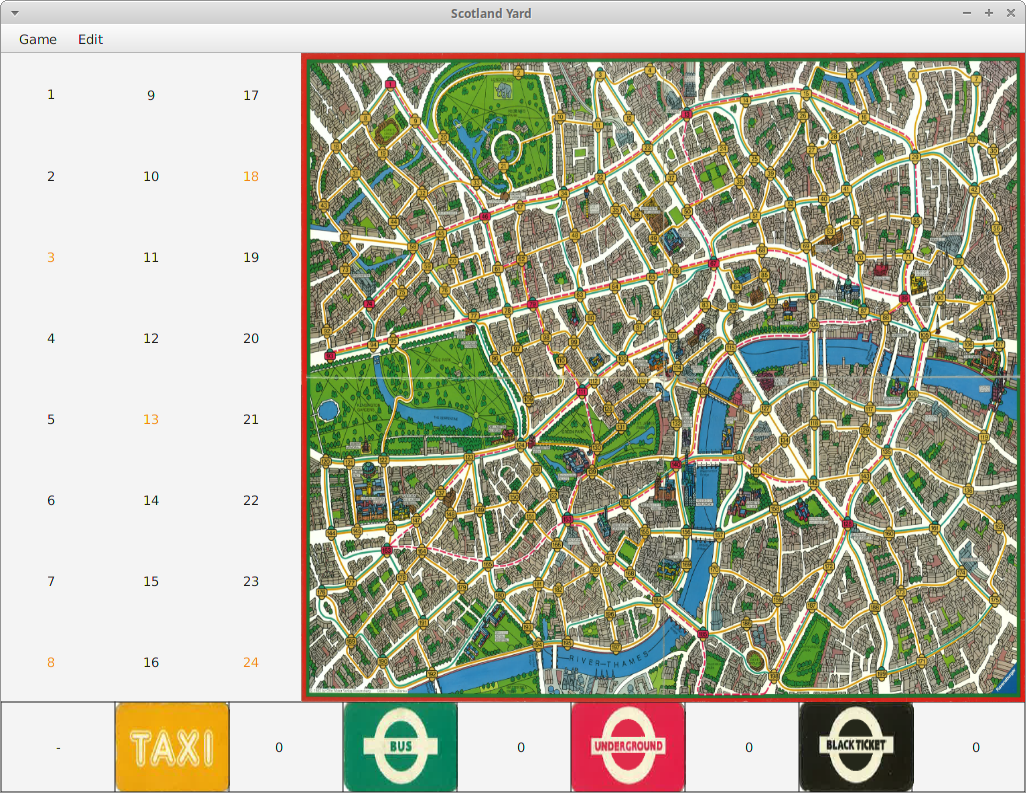
\includegraphics[scale=0.3]{img/benutzerhandbuch/programmstart.png}   
                \caption{Spieloberfläche nach starten des Programmes}
                \label{abb_programmstart}
            \end{figure}
           
            \begin{figure}[H]
                \centering
                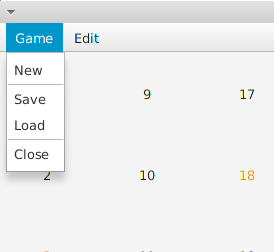
\includegraphics[scale=0.7]{img/benutzerhandbuch/menu_game.png}   
                \caption{Menüpunkt \textit{Game}}
                \label{abb_menuGame}
            \end{figure}
            Abb. \ref{abb_menuGame} zeigt alle verfügbaren Unterpunkte des Menüpunktes \textit{Game}.
            Ein neues Spiel wird durch ein Klick auf \textit{New Game} gestartet.
            Um ein Spiel zu Speichern oder zu laden, wird auf \textit{Save} bzw. \textit{Load} geklickt.
            Das Spiel wird über \textit{Close} beendet.
            \begin{figure}[H]
                \centering
                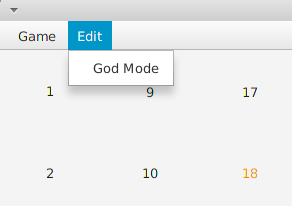
\includegraphics[scale=0.7]{img/benutzerhandbuch/menu_edit.png}   
                \caption{Menüpunkt \textit{Edit}}
                \label{abb_menu_edit}
            \end{figure}
            Wie in Abb. \ref{abb_menu_edit} gezeigt hat der Menüpunkt \textit{Edit} 
            nur einen Unterpunkt \textit{Godmode}.
            Durch einen Klick auf diesen Menüpunkt ist Mister-X dauerhaft auf der Spielkarte zu sehen.
            Durch einen weiteren Klick ist Mister-X wieder versteckt.
             
        \subsection{Neues Spiel starten}
            Um ein neues Spiel zu starten muss auf den Menüpunkt \textit{New Game} geklickt werden (siehe Abbildung \ref{abb_menuGame}).
            Daraufhin öffnet sich ein Fenster welches die Spieleinstellungen abfragt.
            Die Einstellung \textit{MisterX AI?} legt fest, ob Mister-X durch die künstliche Intelligenz (KI)
            oder einen menschlichen Mitspieler gesteuert werden soll. Äquivalent gilt dies für \textit{Detectives AI?}. 
            Zu beachten ist jedoch, dass diese Einstellung für alle Detektive gleichermaßen gilt.
            Über \textit{How many Detectives} lässt sich die Anzahl an Detektiven bestimmen die am Spiel teilnehmen.
            Gültige werte sind hier 3, 4 und 5.

            \begin{figure}[H]
                \centering
                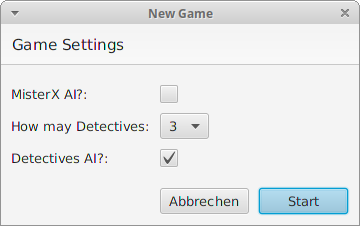
\includegraphics[scale=0.7]{img/benutzerhandbuch/settings.png}   
                \caption{Dialog: Standardeinstellungen für ein neues Spiel}
                \label{abb_settings}
            \end{figure}
            Sobald alle Einstellungen nach Wunsch vorgenommen wurden, kann das Spiel über \textit{Start} gestartet werden.
            Nun werden die verfügbaren Tickets und der Spieler der zurzeit an der Reihe ist angezeigt.
            
            \begin{figure}[H]
                \centering
                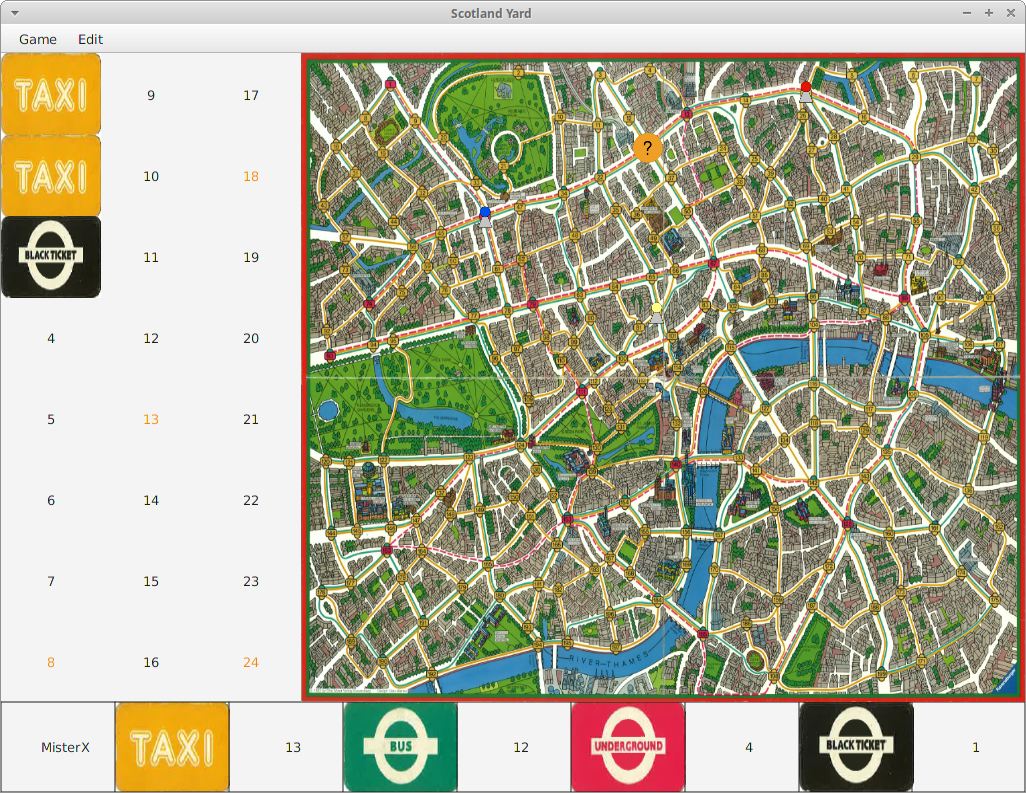
\includegraphics[scale=0.3]{img/benutzerhandbuch/gamerun.png}   
                \caption{Spielfeld nach ein paar Spielzügen}
                \label{abb_settings}
            \end{figure}

            Falls schon ein Spiel gestartet wurde, wird mit einer entsprechenden Meldung davor gewarnt,
            dass das aktuelle Spiel verloren gehen wird.

            \begin{figure}[H]
                \centering
                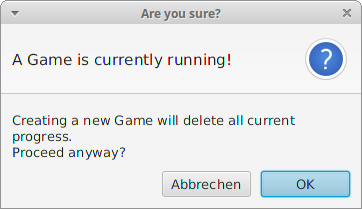
\includegraphics[scale=0.7]{img/benutzerhandbuch/dialognewgame.png}   
                \caption{Warnung: Aktuelles Spiel geht beim starten verloren}
                \label{abb_dialognewgame}
            \end{figure}
            
            
        \subsection{Spielprinzip}
            Die Kernaufgabe des Spiels \textit{Scotland Yard} besteht darin Mister-X zu fangen.
            Dabei Spielen die Detektive gegen Mister-X. Gespielt werden 24 Runden.
            Dabei ist Mister-X für die Detektive nur in bestimmten Runden zu sehen.
            Jeder Spieler startet dabei auf einer zufälligen Startposition.

        \subsubsection{Fahrtenbuch}
            MisterX ist für die Detektive nur in den Spielrunden 3, 8 13 18 und 24 Sichtbar.
            In den anderen Runden ist er verdeckt.
            Dabei wird jedoch jedes verbrauchte Ticket in dem Fahrentenbuch aufgelistet.
            Dadurch können die Detektive mit Hilfe der letzten Zeigeposition von Mister-X die möglichen Zielpositionen errechnen.
        \subsubsection{Spielende}
            Das Spiel ist für die Detektive gewonnen sobald Mister-X gefangen wurde.
            Das heißt, dass einer der Detektiven auf die aktuelle Position von Mister-X gezogen ist.
            Des Weiteren können die Detektive Mister-X auch umkreisen, sodass dieser nicht mehr ziehen kann.
            \begin{figure}[H]
                \centering
                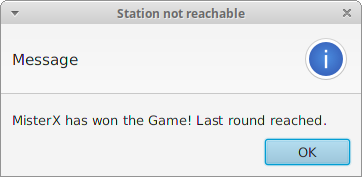
\includegraphics[scale=0.6]{img/benutzerhandbuch/won_lastround.png}   
                \caption{Meldung: Letzte runde erreicht. Mister-X hat gewonnen}
            \end{figure}

            \begin{figure}[H]
                \centering
                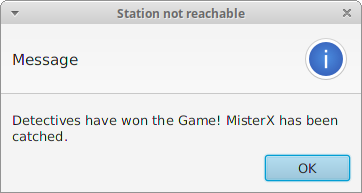
\includegraphics[scale=0.6]{img/benutzerhandbuch/won_catch.png}   
                \caption{Meldung: Mister-X wurde gefangen}
            \end{figure}
            \begin{figure}[H]
                \centering
                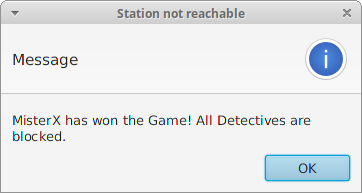
\includegraphics[scale=0.6]{img/benutzerhandbuch/won_blocked.png}   
                \caption{Meldung: Alle Detektive sind blockiert}
            \end{figure}
            Für Mister-X besteht die Chance zu gewinnen dardurch, dass den Detektiven die Tickets ausgehen.
            Zusätzlich kann Mister-X auch gewinnen falls die letzte Runde erreicht worden ist und dieser noch nicht gefangen wurde.
        \subsubsection{Tickets}
            Um von einer Station zur anderen zu gelangen benötigen die Spieler Tickets für die Verkehrsmittel.
            Dabei stehen den Detektiven 10 Taxi-, 8 Bus- und 4 U-Bahntickets zur Verfügung.
            Mister-X hingegegen stehen  10 Taxi-, 8 Bus-, 4 U-Bahn- und 2 Blacktickets zur Verfügung.
            Eine Besonderheit des Blacktickets ist hierbei, dass dieses für alle Verkehrsmittel, also auch für das Boot, gilt.
            Zusätzlich werden alle verbrauchten Tickets der Detektive, Mister-X gutgeschrieben.
            Somit kann diesem nie die Tickets ausgehen.
        \subsubsection{Züge}
            Alle Spieler die auf eine Station ziehen wollen, benötigen jeweils das richtige bzw. noch genügend Tickets um die Station zu erreichen.
            Hat ein Spieler nicht mehr genügend Tickets übrig, muss dieser für diese Runde aussetzen.
            \newline
            \newline
            Um die Spielerfigur zu bewegen, wird in die Nähe der gewünschten Zielstationtation geklickt.
            Kann die Zielstation durch mehrere Verkehrsmittel erreicht werden, wird ein Dialog zur Auswahl
            des gewünschten Tickets geöffnet. (siehe Abb. \ref{abb_dialogchooseticket})

            \begin{figure}[H]
                \centering
                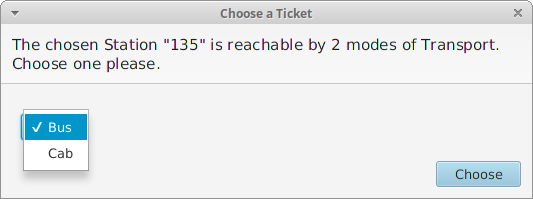
\includegraphics[scale=0.6]{img/benutzerhandbuch/dialogchooseticket.png}   
                \caption{Dialog: Ticketauswahl}
                \label{abb_dialogchooseticket}
            \end{figure}
            Falls auf eine Station gezogen werden soll die nicht erreichbar bzw. blockiert
            ist, oder der Spieler nicht genügend Tickets übrig hat, erscheint eine entsprechende Meldung. 
            (siehe folgende Abbildungen)
            \begin{figure}[H]
                \centering
                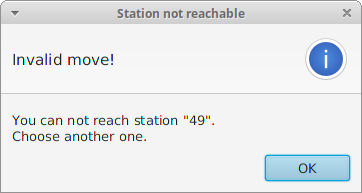
\includegraphics[scale=0.7]{img/benutzerhandbuch/dialog_invalid_move.png}   
                \caption{Meldung: Station nicht erreichbar}
                \label{abb_dialog_invalid_move}
            \end{figure}

            \begin{figure}[H]
                \centering
                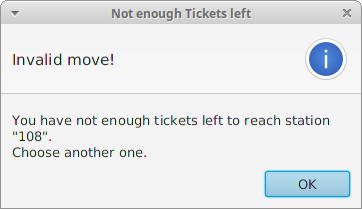
\includegraphics[scale=0.7]{img/benutzerhandbuch/dialog_not_enough_tickets.png}   
                \caption{Meldung: Ungenügend Tickets}
                \label{abb_dialog_not_enough_tickets}
            \end{figure}

        \subsection{Spiel speichern}
                Um ein laufendes Spiel zu speichern, wird auf den Menüpunkt \textit{Save} des Oberpunktes \textit{Game} geklickt.
                Dadurch wird ein Datei-Navigator zur Auswahl des Speicherortes und des Namens des Spielstandes geöffnet.
                Hierbei ist zu beachten, dass die Datei die Endung \texttt{.sy} beinhalten muss.
                Die Endung wird nicht automatisch hinzugefügt, wird jedoch für das Laden eines Spielstandes benötigt.

                Falls noch kein Spiel gestartet worden ist, schlägt das Speichern mit einer entsprechenden Meldung fehl.
                \begin{figure}[H]
                    \centering
                    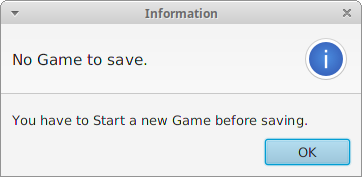
\includegraphics[scale=0.7]{img/benutzerhandbuch/dialog_no_game_to_save.png}   
                    \caption{Meldung: Speicherung eines nicht existierenden Spielstandes}
                    \label{abb_dialog_no_game_to_save}
                \end{figure}

                \begin{figure}[H]
                    \centering
                    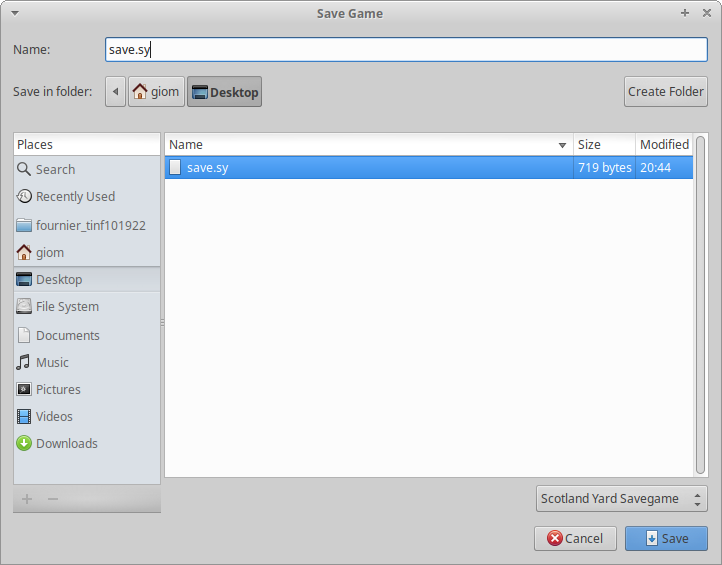
\includegraphics[scale=0.4]{img/benutzerhandbuch/dialog_save_filechooser.png}   
                    \caption{Datei Auswahl zum speichern des Spielstandes}
                    \label{abb_dialog_save_filechooser}
                \end{figure}

                Falls die Datei schon existiert und damit eine Überschreibung eines Spielstandes droht,
                öffnet sich eine Meldung.
                \begin{figure}[H]
                    \centering
                    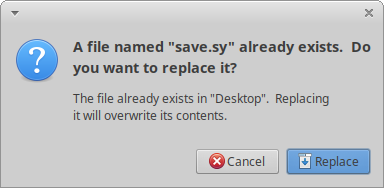
\includegraphics[scale=0.7]{img/benutzerhandbuch/dialog_save_replace.png}   
                    \caption{Meldung: Überschreibung eines Spielstandes}
                    \label{abb_dialog_save_replace}
                \end{figure}

                
        \subsection{Spiel laden}
            Um ein Spiel zu laden, wird auf den Menüpunkt \textit{Load} des Oberpunktes \textit{Game} geklickt.
            Dadurch öffnet sich ein Datei-Navigator der dazu auffordert eine Datei auszuwählen aus der,
            der Spielstand geladen werden soll. Dabei ist zu beachten, dass der Datei-Navigator nur Dateien einblendet die eine
            Endung \texttt{.sy} beinhalten. Falls zur Zeit des Ladens ein Spiel am laufen ist, erscheint eine
            Meldung, dass das laufende Spiel dabei verloren gehen wird.

            \begin{figure}[H]
                \centering
                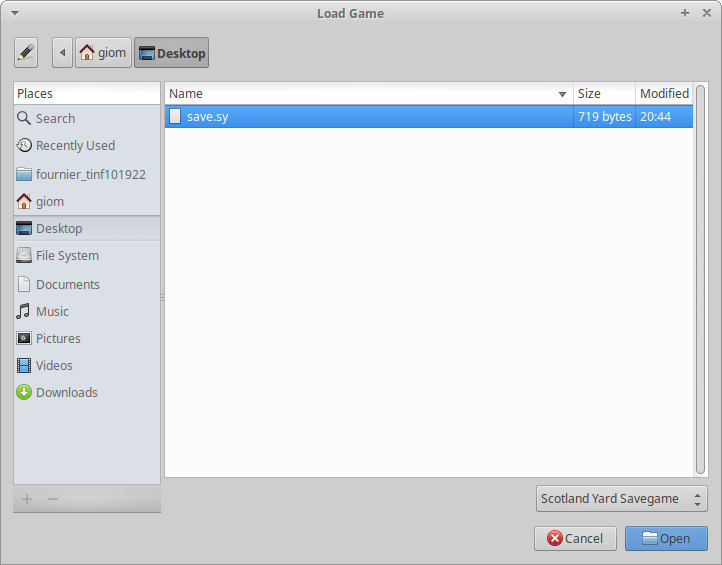
\includegraphics[scale=0.4]{img/benutzerhandbuch/dialog_load.png}   
                \caption{Datei-Navigator zum laden eines Spielstandes}
            \end{figure}

            \begin{figure}[H]
                \centering
                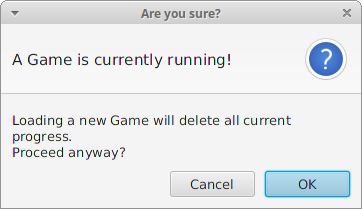
\includegraphics[scale=0.7]{img/benutzerhandbuch/dialog_load_override.png}   
                \caption{Meldung: Der aktuelle Spielstand wird gelöscht}
            \end{figure}
                
        \subsection{Spiel beenden}
            Um ein Spiel zu beenden, wird auf den Menüpunkt \textit{Close} des Oberpunktes \textit{Game} geklickt.
            Falls zur Zeit des Beendens ein Spiel am laufen ist, erscheint eine Meldung, dass das laufende Spiel dabei verloren gehen wird.
        \subsection{Godmode}
            Beim Klicken auf den Menüpunkt \textit{Godmode} des Oberpunktes \textit{Edit}, wird der Godmode aktiviert.
            Dadurch ist Mister-X auch ausserhalb seiner Zeigerunden sichtbar. Durch erneutes Klicken auf den Menüpunkt
            wird dieser Modus deaktiviert.

        \subsection{Spiellog}
            Um das Spiel im nachhinein analysieren zu können, schreibt das Programm alle nötigen Informationen in eine Datei
            namens \textit{game.log}. Diese Datei wird vor jedem Spiel automatisch angelegt oder überschrieben falls diese noch
            nicht existiert. Dabei wird die Struktur im Kapitel \ref{log} erläutert.
    \section{Fehlermeldungen}
        Das Programm zeigt im Falle eines Fehlers folgende Fehler an.
        \newline
        \newline
        Folgende Abbildung zeigt die Fehlermeldung die erscheint, wenn das zu ladende Spielfeld
        fehlerhaft formatiert ist. Um den Fehler zu beseitigen muss sichergestellt werden,
        dass die Spielfelddatei eine valide \textit{JSON}-Struktur ist und diese alle Felder besitzt
        die in \ref{Spielfeldsdatei} beschrieben sind. Zusätzlich müssen die Datentypen stimmen.
        \begin{figure}[H]
            \centering
            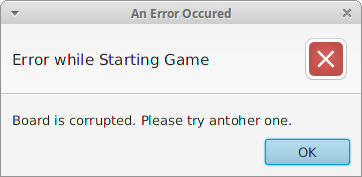
\includegraphics[scale=0.7]{img/benutzerhandbuch/error_boardcorrupted.png}   
            \caption{Fehler: Spielfeld falsch formatiert}
        \end{figure}
        Folgende Abbildung zeigt die Fehlermeldung die erscheint wenn das zu ladene Spielfeld fehlerhafte
        Werte hält. Um den Fehler zu beseitigen muss sichergestellt werden, dass die Werte korrekt sind.
        Dazu zählen, Stationsidentifikationsnummern die auch wirklich existieren.
        \begin{figure}[H]
            \centering
            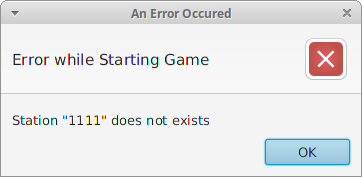
\includegraphics[scale=0.7]{img/benutzerhandbuch/error_boardvalue.png}   
            \caption{Fehler: Spielfeld beinhaltet ungültige Werte}
        \end{figure}
        Folgende Abbildung zeigt die Fehlermeldung die erscheint wenn das zu ladene Spielfeld nicht existiert.
        Um den Fehler zu beseitigen muss sichergestellt werden, dass die Datei im \textit{JAR} unter dem Ordner \textit{Logik/Board}
        liegt und \textit{network.json} heißt.
        \begin{figure}[H]
            \centering
            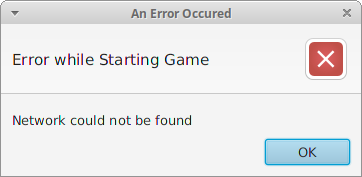
\includegraphics[scale=0.7]{img/benutzerhandbuch/error_nosuchfile.png}   
            \caption{Fehler: Spielfeld nicht gefunden}
        \end{figure}
        Folgende Abbildung zeigt die Fehlermeldung die erscheint wenn die zu ladene Spielstandsdatei fehlerhafte
        Formatiert ist. Um den Fehler zu beseitigen muss sichergestellt werden,
        dass die Spielstandsdatei eine valide \textit{JSON}-Struktur ist und diese alle Felder besitzt
        die in \ref{Spielstandsdatei} beschrieben sind. Zusätzlich müssen die Datentypen stimmen.
        \begin{figure}[H]
            \centering
            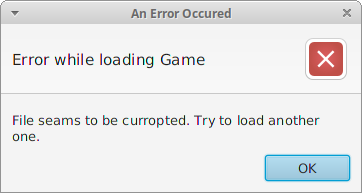
\includegraphics[scale=0.7]{img/benutzerhandbuch/error_savecorrupted.png}   
            \caption{Fehler: Spielstandsdatei falsch formatiert}
        \end{figure}
        Folgende Abbildung zeigt die Fehlermeldung die erscheint wenn das zu ladene Spielstandsdatei fehlerhafte
        Werte hält. Um den Fehler zu beseitigen muss sichergestellt werden, dass die Werte korrekt sind.
        Dazu zählen, keine Negative Tickets und Stationsidentifikationsnummern die auch wirklich existieren.
        \begin{figure}[H]
            \centering
            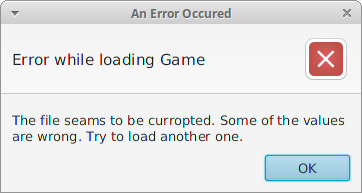
\includegraphics[scale=0.7]{img/benutzerhandbuch/error_savevalue.png}   
            \caption{Fehler: Spielstandsdatei beinhaltet falsche Werte}
        \end{figure}


    \section{Datenstrukturen}\label{Datenstrukturen}
        \subsubsection{Spielfeldsdatei}\label{Spielfeldsdatei}
            Die Datei indem das Spielfeld gespeichert ist, ist im \textit{JSON}-Format kodiert.
            Im Grunde beinhaltet diese ein homogenes \textit{Json}-Array aus \textit{Json}-Objekten.
            Dabei bilden die Objekte eine Station mit Identifikationsnummer, Position und verfügbaren Nachbarstationen, erreichbar über ein Verkehresmittel.
            Die Datenstruktur sieht dabei wie folgt aus:

            \begin{itemize}
                \item stations - Array aus folgenden Objekt
                    \begin{itemize}
                        \item identifier
                        \item position
                            \begin{itemize}
                                \item x: Koorindate als double
                                \item y: Koorindate als double
                            \end{itemize}
                        \item tube: Ein Array aus Identifikationsnummern.
                        \item bus: Ein Array aus Identifikationsnummern
                        \item cab: Ein Array aus Identifikationsnummern
                        \item boat: Ein Array aus Identifikationsnummern
                    \end{itemize}
            \end{itemize}

    \subsubsection{Spielstandsdatei}\label{Spielstandsdatei}
        Die Datei indem der Spielstand gespeichert ist, ist im \textit{JSON}-Format kodiert.
        Dabei beinhaltet die Datei folgende Felder:
        \begin{itemize}
            \item MisterX: Object
                \begin{itemize}
                    \item ai: boolean
                    \item possibleTargets: int-Array
                    \item lastShownPos: int
                    \item currPos: int
                    \item remainingTickets: int-Array
                    \item journeyBoard: int-Array
                \end{itemize}
            \item detectives: Object-Array
                \begin{itemize}
                    \item noOfDetectives: int
                    \item ai: boolean
                    \item players: Object-Array in der länge von \textit{noOfDetectives}
                        \begin{itemize}
                            \item position: int
                            \item remainingTickets: int-Array
                        \end{itemize}
                \end{itemize}
            \item whosTurn: int
            \item currRoundNo: int
            \item gameIsWon: boolean
        \end{itemize}

    \subsubsection{Spiellog}\label{log}
        Die logdatei ist in einer Struktur aufgebaut die, die Werte durch Kommata trennt.
        Dabei stellt die erste Zeile die Spielkonfiguration dar.
        \begin{itemize}
            \item die Anzahl der Detektive (ganze Zahl)
            \item ob MisterX von der KI gesteuert wird (true oder false)
            \item ob die Detektive von der KI gesteuert werden (true oder false)
            \item die Startposition von MisterX
            \item die Startpositionen aller teilnehmenden Detektive
        \end{itemize}
        Die darauffolgenden Zeilen repräsentieren ein Zug durch einen Spieler:
        \begin{itemize}
            \item welcher Spieler zieht (ganze Zahl ab 1 für die Detektive, 0 für MisterX)
            \item bisherige Station
            \item neue Station
            \item restliche Tickets für U-Bahn, Bus, Taxi, Boot
            \item welche der Taktiken wurde gewählt (bei einem menschlichen Spielzug = 0)
            \item die Bewertung der Taktik
        \end{itemize}
        Die letzte Zeile besagt, ob und von wem ein Spiel gewonnen wurde.
        Dabei steht die 0 für Mister-X und die 1 für die Detektive.
      